\documentclass[xetex]{beamer}


\mode<presentation> {
%  \usetheme{Singapore}
  \usetheme{Frankfurt}
  \setbeamercovered{transparent}
}

\usepackage{xunicode}
\usepackage{xltxtra}
\usepackage[czech]{babel}
\usepackage{palatino}
\usepackage{graphicx}
\usepackage{tikz}
\usepackage{pgflibraryarrows}
\usepackage{pgflibrarysnakes}

\title{CryptoParty\\Základy počítačové bezpečnosti\\pro začátečníky}

\author{Ondřej Profant}
\institute[Piráti]{Česká pirátská strana}
\date{\today}

\begin{document}

\begin{frame}
  \titlepage
\end{frame}

\begin{frame}
  \frametitle{Osnova}
  \tableofcontents
\end{frame}	

\section{Počítač}
\begin{frame}
 \frametitle{Přístup}
 \begin{itemize}
  \item Počítač není nepřítel.
  \item Počítač je stroj.
  \item Software je to s čím pracujete.
  \item Software již může být váš nepřítel - naštěstí ho lze vyměnit.
  \item Pokud vám něco nejde:
   \begin{enumerate}
    \item Zkuste se naučit pracovat s danou aplikací.
    \item Zkuste alternativní aplikace.
   \end{enumerate}
 \end{itemize}
\end{frame}
%TODO

\section{Hesla}

\begin{frame}
 \frametitle{Hesla}
 Zásady silného hesla:
 \begin{itemize} 
   \item přiměřeně dlouhé
   \item více druhů znaků (písmena, čísla, jiné znaky)
   \item nepoužívat existující slova 
   \item nepoužívat všude stejné heslo (alespoň několik stupňů)
 \end{itemize}
\end{frame}

\begin{frame}
	\frametitle{Hesla}
	
\includegraphics[scale=0.5]{pic/heslo.jpg}
\end{frame}


\begin{frame}
 \frametitle{Hesla}
 Jak to splnit:
 \begin{itemize} 
   \item kombinovat, modifikovat
   \item prokládat
   \item vyhodnocovat riziko
   \item správci hesel
 \end{itemize} 

Silné heslo nemusí být složité.
\end{frame}

\section{Operační systém}

\subsection{Pravidelné aktualizace}

\begin{frame}
	\frametitle{Pravidelné aktualizace} 
	\begin{itemize}
		\item Každý systém poskytuje bezpečnostní aktualizace.
		\item Tyto aktualizace se opravdu vyplatí nainstalovat.
		\item Tyto aktualizace jsou zpravidla zdarma.
	\end{itemize}
\end{frame}

\begin{frame}
	\frametitle{Pravidelné aktualizace 2} 
	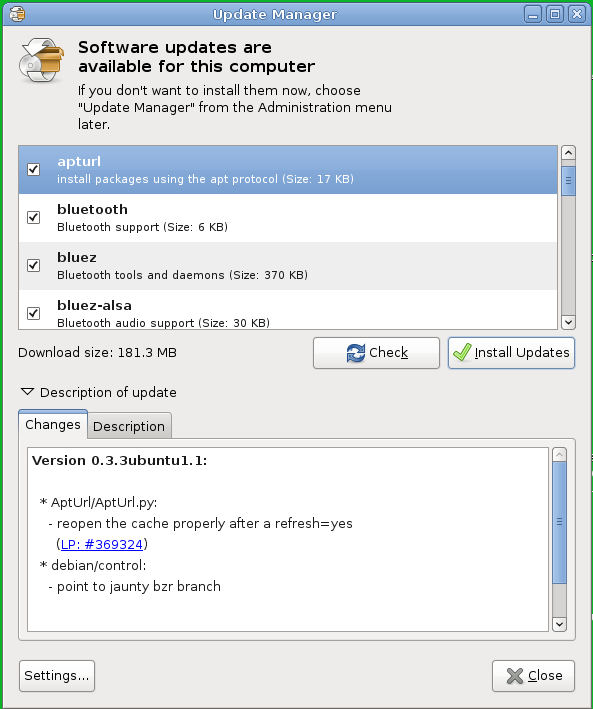
\includegraphics[scale=0.3]{pic/gnome-update.png}
\end{frame}

\begin{frame}
	\frametitle{Pravidelné aktualizace 3} 
	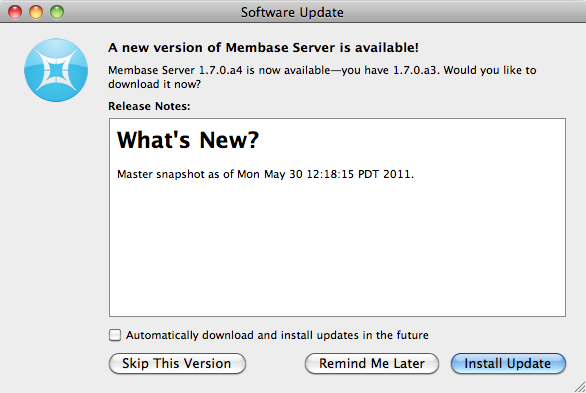
\includegraphics[scale=0.5]{pic/macosx-update.png}
\end{frame}

\begin{frame}
 	\frametitle{Pravidelné aktualizace 4} 
	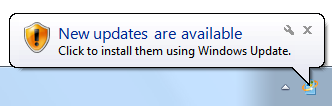
\includegraphics{pic/win-update.png}
\end{frame}

\subsection{Uživatelské účty}

\begin{frame}
	\frametitle{Uživatelské účty} 
	\begin{itemize} 
   		\item Uživatelské účty jsou praktická věc!
	   	\item Oddělují prostředí.
   		\item Zabezpečují základní soukromí.
	\end{itemize} 
\end{frame}

\subsection{Výběr OS}

\begin{frame}
 	\frametitle{Operační systém} 
 	\begin{itemize} 
   		\item Existuje více druhů operačních systémů
   		\item S různým zaměřením a různým stylem používání
 	\end{itemize} 

	\bigskip

	Příklady pro desktop: Windows 7, Windows 8, Mac OS X, Ubuntu, Fedora, FreeBSD, Chrome OS

	\bigskip

	Příklady pro mobily: Windows Phone, iOS, Android, Sailfish OS 
\end{frame}

\section{Internetové prohlížeče}

\begin{frame}
	\frametitle{Internetové prohlížeče} 
	\begin{itemize} 
   		\item Existuje více prohlížečů
		\item Liší se kvalitou, rychlostí
   		\item a mnohdy bezpečností a přístupem k ni
	\end{itemize} 

	\bigskip

	Příklady: Internet Explorel, Mozila Firefox, Google Chrome
\end{frame}

\subsection{Anonymní mód}

\begin{frame}
	\frametitle{Anonymní mód} 
	\begin{itemize} 
		\item Neukládá data do počítače.
		\item Nepoužívá data již uložená (např. cookies).
		\item Slouží k základní anonymizaci, ale ne moc podrobné.
		\item Nejedná se o anonymizér.
	\end{itemize} 
\end{frame}

\begin{frame}
 	\frametitle{Anonymní mód -- Firefox} 
	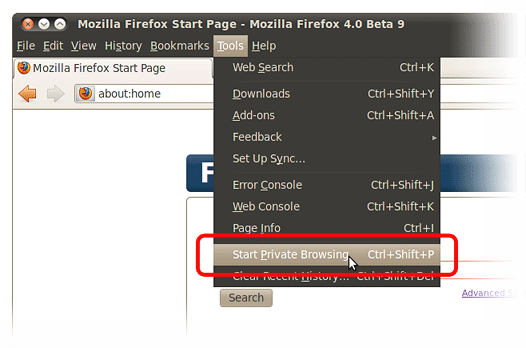
\includegraphics[scale=0.5]{pic/firefox-private2.png}
\end{frame}

\begin{frame}
 	\frametitle{Anonymní mód -- Chrome} 
	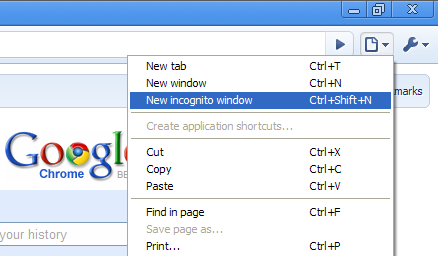
\includegraphics[scale=0.6]{pic/chromium-private2.png}
\end{frame}

\begin{frame}
	\frametitle{Anonymizéry} 
	\begin{itemize} 
		\item např. Tor
		\item ke stažení přímo předpřipravený prohlížeč:\\
\begin{scriptsize}https://www.torproject.org/projects/torbrowser.html.en\end{scriptsize}
		\item jiné řešení může být např. VPN
	\end{itemize} 
\end{frame}

\begin{frame}
	\frametitle{Anonymizéry} 
	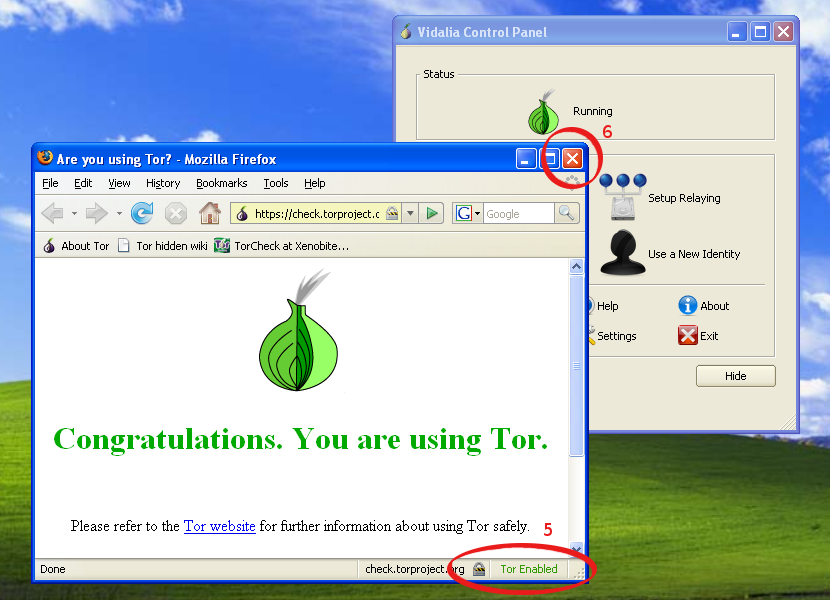
\includegraphics[scale=0.4]{pic/tor-xp.png}
\end{frame}

\subsection{Certifikáty a zabezpečení stránek}

\begin{frame}
	\frametitle{Certifikáty a zabezpečení stránek} 
	\begin{itemize} 
   		\item neodklikávajte bez rozmyslu
	\end{itemize} 
\end{frame}


\begin{frame}
	\frametitle{Certifikáty a zabezpečení stránek} 
	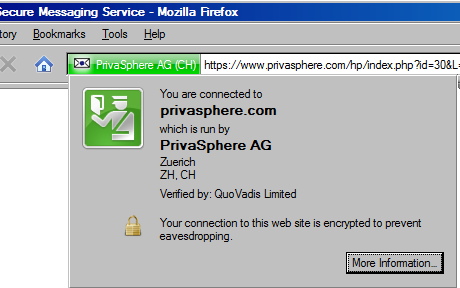
\includegraphics[scale=0.5]{pic/firefox-trust.png}
\end{frame}

\subsection{Pluginy, addony}

\begin{frame}
	\frametitle{Prohlížeče -- pluginy, addony}
	\begin{itemize} 
   		\item Nebezpečné.
  	 	\item Ztráta výkonu.
  	 	\item Odinstalujte, co nepoužíváte.
	\end{itemize} 
\end{frame}

\section{Šifrování}

\subsection{Archívy}

\begin{frame}
	\frametitle{Archívy} 
	\begin{itemize} 
   		\item Archívy slouží primárně ke komprimaci (zmenšení) dat.
  	 	\item Nicméně většinou dovolují i šifrovat.
	\end{itemize} 
\end{frame}

\begin{frame}
	\frametitle{Odbočka: šifrování vs. ,,heslování''} 
	\begin{itemize} 
   		\item Kvalitní šifrování je z podstaty bezpečné.
   		\item ,,Heslování'' může znamenat pouze ochrana heslem.
	\end{itemize} 
\end{frame}

\begin{frame}
 \frametitle{Archívy} 
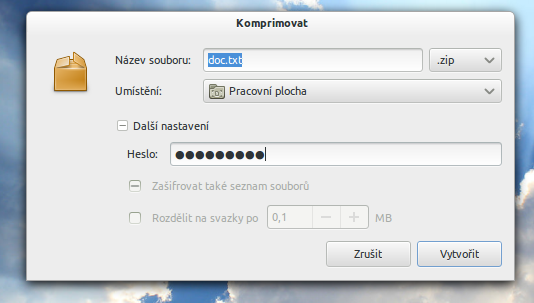
\includegraphics[scale=0.6]{pic/zip-pass.png}
\end{frame}

\begin{frame}
 \frametitle{Šifra}
 Opravdová šifra:

 \bigskip

 openssl aes-256-cbc -in <input> -out <output>.aes

 \bigskip

 openssl aes-256-cbc -d -in <input>.aes -out <output>
\end{frame}

\section{Cloudy}

\begin{frame}
 \frametitle{Cloudy} 
\begin{itemize} 
   \item Uložiště dat mimo váš počítač
   \item Obvykle mimo konkrétní počítač
   \item Již z principu založeno na důvěře poskytovateli
   \item Samozřejmě jsou lepší a horší řešení (např. Mega šifruje na straně klienta)
 \end{itemize} 
\end{frame}

\section{Další témata}
\begin{frame}
 \frametitle{Další témata}
 \begin{itemize}
  \item Steganografie: metoda ukytí správy v obrázku
  \item OTR: šifrování IM komunikace
  \item Bitcoin: virtuální decentralizovaná kryptoměna
  \item VPN: soukromá síť skrz internet
  \item TOR: anonymizační síť
  \item dalšín témata: DPI, Cryptohandbook, Truecrypt
 \end{itemize}
\end{frame}

\section{Závěr}

\begin{frame}
  \frametitle{Závěr}
	Děkuji za pozornost.

	\bigskip
	
	Doplňující otázky?

	\bigskip
	
	Další Cryptoparty?

	\bigskip

	\url{http://www.cryptoparty.cz}

	\bigskip

	\scriptsize
Copyleft Ondřej Profant, 2012. Všechna práva vyhlazena. Sdílejte, upravujte a~nechte sdílet za stejných podmínek. 

Prezentace v~úplné formě\footnote{i se zdrojovými kódy} na \url{http://github.com/kedrigern/prezentace-cs}
\end{frame}

\end{document}
